\section{Dữ liệu 1: Mô hình hồi quy đa biến}

\subsection*{Giới thiệu bộ dữ liệu}
Bộ dữ liệu được tìm thấy trên trang Kaggle - một cộng đồng trực tuyến về khoa học dữ liệu và học máy. Đó là bộ dữ liệu \textbf{Chi phí Y tế Cá nhân} \footnote{\url{https://www.kaggle.com/mirichoi0218/insurance}} (\textit{Medical Cost Personal Datasets}). Đây là một bộ dữ liệu được lấy ra từ cuốn \textit{Machine Learning with R} của Brett Lantz, một cuốn sách giới thiệu về học máy bằng R.

Bộ dữ liệu ghi lại các thông tin về thông tin của người đăng kí bảo hiểm và chi phí mà bảo hiểm y tế phải chi trả cho cá nhân đó. Bộ dữ liệu có 1338 quan trắc, gồm 7 biến sau:
\begin{enumerate}
	\item \textbf{Age}: tuổi
	\item \textbf{Sex}: giới tính
	\item \textbf{BMI}: chỉ số đo cân nặng, sử dụng tỷ lệ giữa cân nặng và chiều cao ($kg / m$), chỉ số BMI lý tưởng là từ 18.5 đến 24.9.
	\item \textbf{Children}: số lượng trẻ em được bao gồm trong bảo hiểm y tế của người đăng kí.	
	\item \textbf{Smoker}: 1 nếu người đó có hút thuốc, ngược lại là 0.
	\item \textbf{Region}: vùng miền ở US, bao gồm Đông Bắc (\textit{northeast}), Đông Nam (\textit{southeast}), Tây Nam (\textit{southwest}), Tây Bắc (\textit{northwest}).
	\item \textbf{Charges}: Chi phí y tế của cá nhân được chi trả bởi bảo hiểm y tế.
\end{enumerate}

Nhận thấy biến $region$ có bốn giá trị, để thuận tiện cho việc hồi quy mô hình đa biến, chúng ta cần phải tách $region$ thành ba biến giả lần lượt là $region\_ne$ - vùng Đông Bắc, $region\_se$ - vùng Đông Nam và $region\_sw$ - vùng Tây Nam, nếu không nằm trong 3 vùng này thì nó là vùng Tây Bắc. Vậy bộ dữ liệu có tất cả 9 biến.

Kiểm tra sự trùng lặp dữ liệu trong bộ dữ liệu, ta có kết quả từ phầm mềm R ở hình \ref{fig-a1:dataset-duplicated}, thấy rằng chỉ tồn tại một dữ liệu bị trùng, ta tiến hành loại bỏ dữ liệu này. Vậy bộ dữ liệu có 1337 quan trắc.
\begin{figure}[H]
	\centering
	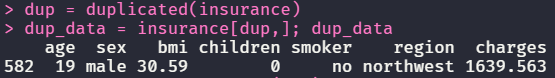
\includegraphics[width=0.7\linewidth]{images/A1/dataset-duplicated}
	\caption{Dữ liệu bị trùng lặp}
	\label{fig-a1:dataset-duplicated}
\end{figure}

Một vài quan trắc đầu tiên trong bộ dữ liệu được thể hiện trong hình \ref{fig-a1:head-dataset} và số chiều của nó: 1337 dòng (quan trắc) và 9 cột (biến).
\begin{figure}[H]
	\centering
	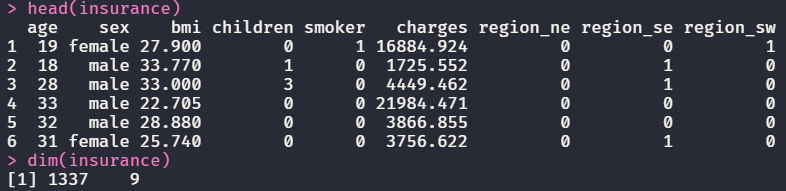
\includegraphics[width=0.8\linewidth]{images/A1/head-dataset}
	\caption{Một vài quan trắc đầu tiên và số chiều của bộ dữ liệu}
	\label{fig-a1:head-dataset}
\end{figure}

Phân bố của 7 biến ban đầu với biến $region$ ở hình \ref{fig-a1:plot-vars}.
\begin{figure}[H]
	\centering
	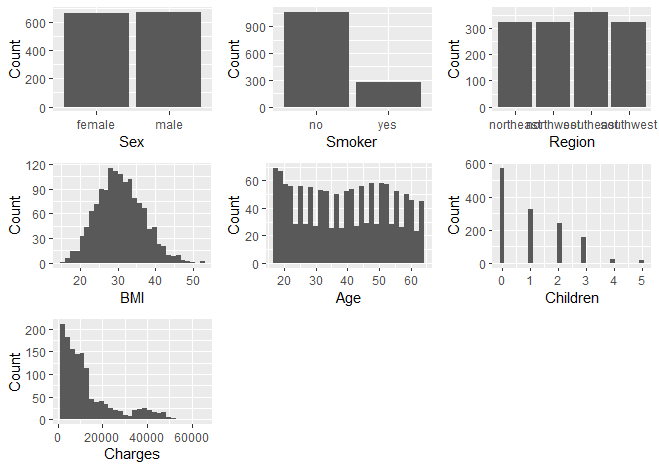
\includegraphics[width=0.8\linewidth]{images/A1/plot-vars}
	\caption{Phân bố của 7 biến ban đầu}
	\label{fig-a1:plot-vars}
\end{figure}

\subsection*{Phân tích và chọn mô hình}

\subsection*{Nhận xét và kết luận}